\documentclass[12pt,openright,oneside,a4paper,chapter=TITLE,sumario=tradicional,english,brazil]{abntex2}

\usepackage[T1]{fontenc}
\usepackage[utf8]{inputenc}
\usepackage{lmodern}
\usepackage{amsmath,amssymb}
\usepackage{graphicx}
\usepackage{booktabs}
\usepackage{array}
\usepackage{xcolor}
\usepackage{listings}
\usepackage{microtype}
\usepackage{tikz}
\usetikzlibrary{arrows.meta,positioning}
\usepackage{pgfplots}
\pgfplotsset{compat=1.16}

\lstset{basicstyle=\ttfamily\footnotesize,frame=single,breaklines=true,columns=fullflexible,
  showstringspaces=false,backgroundcolor=\color{black!3}}

\titulo{Verificação formal de um controlador neural em malha fechada (\emph{cart-pole}): resultados com BMC (ESBMC) e com IC3/PDR}
\autor{Matheus Serrão Uchoa}
\local{Manaus}
\data{2026}
\instituicao{Universidade Federal do Amazonas -- UFAM\par Programa de Pós-Graduação (Mestrado)}
\tipotrabalho{Relatório de resultados}
\preambulo{Relatório técnico de resultados do projeto de verificação formal de controladores neurais quantizados, comparando \emph{Bounded Model Checking} (ESBMC) e \emph{model checking} indutivo (IC3/PDR) sobre o ator DDPG do problema do pêndulo invertido sobre carro.}

\hypersetup{hidelinks,pdfauthor={Matheus Serrão Uchoa},pdftitle={Verificação formal de controlador neural em malha fechada}}
\setlength{\parindent}{1.3cm}
\setlength{\parskip}{0.2cm}

\newcommand{\vtag}[1]{\textbf{#1}}

\begin{document}
\selectlanguage{brazil}
\frenchspacing

\begin{capa}
  \begin{center}
    {\ABNTEXchapterfont\large\imprimirinstituicao}
    \vfill
    {\ABNTEXchapterfont\large\imprimirautor}
    \vfill
    \begin{center}
      \ABNTEXchapterfont\bfseries\Large\imprimirtitulo
    \end{center}
    \vfill
    {\large\imprimirlocal\par\imprimirdata}
    \vspace*{1cm}
  \end{center}
\end{capa}

\begin{folhaderosto}
  \begin{center}
    {\ABNTEXchapterfont\large\imprimirautor}
    \vfill
    \begin{center}
      \ABNTEXchapterfont\bfseries\Large\imprimirtitulo
    \end{center}
    \vfill
    \hspace{.45\textwidth}
    \begin{minipage}{.5\textwidth}
      \SingleSpacing\small\imprimirpreambulo
    \end{minipage}
    \vfill
    {\large\imprimirlocal\par\imprimirdata}
    \vspace*{1cm}
  \end{center}
\end{folhaderosto}

\begin{resumo}
Este relatório consolida os resultados da verificação formal de um controlador neural em malha fechada: o ator de um agente DDPG (arquitetura $4{\to}24{\to}24{\to}1$, 745 parâmetros, quantizado em ponto fixo Q8.8) que equilibra o pêndulo invertido sobre carro (\emph{cart-pole}). Duas famílias de método são comparadas. A primeira usa \emph{Bounded Model Checking} (BMC) com o ESBMC 6.8.0 sobre \emph{harnesses} em C; ela decide propriedades de um e de dois passos, encontra contraexemplos concretos e reproduzíveis, mas o custo cresce de $0{,}3$~s ($K{=}1$) para $909$~s ($K{=}4$) e a prova de segurança para horizonte ilimitado fica fora de alcance. A segunda traduz a malha fechada para um sistema de transição (Verilog $\to$ AIGER, 904\,242 portas AND, 65 \emph{latches}) e aplica IC3/PDR (ABC); ela produz uma prova ilimitada num modelo sintético com batente mecânico, mas não decide o ator real: o PDR parou no \emph{frame}~2 após 1800~s, o BMC do ABC alcançou 5 \emph{frames} e um motor independente em nível de palavra (Z3/Spacer) também não decidiu. A validação do pipeline mostra que a tradução é equivalente ao C por análise de intervalos e por prova SAT composicional em 49 de 50 blocos, que o pipeline reprova três mutantes comprovadamente inseguros e que as lacunas restantes são declaradas. O relatório \textbf{não} afirma que o controlador real seja seguro para sempre: afirma o que foi provado, o que foi refutado e o que permanece indeciso.

\vspace{\onelineskip}
\noindent\textbf{Palavras-chave}: verificação formal; \emph{model checking}; ESBMC; IC3; PDR; redes neurais quantizadas; \emph{cart-pole}; DDPG.
\end{resumo}

\pdfbookmark[0]{\contentsname}{toc}
\tableofcontents*
\cleardoublepage
\listoffigures*
\cleardoublepage
\listoftables*
\cleardoublepage

\textual

\chapter{Introdução}

Controladores baseados em redes neurais são funções não lineares de alta dimensão. Testá-los por simulação cobre apenas as trajetórias amostradas; a pergunta de segurança, porém, é universal: \emph{para todo estado inicial admissível, o pêndulo nunca ultrapassa 12$^\circ$?} Este relatório responde, com dados medidos, até onde duas técnicas de \emph{model checking} conseguem decidir essa pergunta para o ator DDPG real.

\section{Objetivo}

Apresentar, de forma detalhada e auditável, (i) os resultados do \emph{cart-pole} verificado com BMC no ESBMC; (ii) os resultados do pipeline IC3/PDR sobre a mesma malha fechada; (iii) a validação desse pipeline; e (iv) o que, de fato, está provado e o que não está.

\section{Convenção de vereditos}

Todo resultado deste texto cai em exatamente uma de quatro categorias, e nenhuma é substituída por outra:

\begin{itemize}
  \item \vtag{Provado}: o motor concluiu que a propriedade vale (no escopo e na codificação declarados);
  \item \vtag{Contraexemplo}: o motor exibiu uma execução concreta que viola a propriedade;
  \item \vtag{Indeciso}: o motor excedeu o limite de tempo ou de memória. \textbf{Indeciso não é seguro e não é inseguro};
  \item \vtag{Modelo não validado}: o resultado vale para o modelo traduzido; a equivalência com o artefato real tem lacunas declaradas.
\end{itemize}

\section{Organização}

O Capítulo~\ref{cap:fund} reúne a fundamentação. O Capítulo~\ref{cap:esbmc} apresenta o \emph{cart-pole} com ESBMC. O Capítulo~\ref{cap:ic3} apresenta a rota IC3/PDR. O Capítulo~\ref{cap:valid} descreve a validação do pipeline. O Capítulo~\ref{cap:disc} discute o alcance e a originalidade. O Capítulo~\ref{cap:concl} conclui. Os apêndices trazem logs brutos e instruções de reprodução.

\paragraph{Ambiente.} As medições do Capítulo~\ref{cap:valid} e as reexecuções do Capítulo~\ref{cap:ic3} usaram Yosys 0.33 (ABC embutido), Z3 4.8.12, contêiner Ubuntu 24.04, Intel i7-14700 (28 \emph{threads}) e 32~GB de RAM. As medições do ESBMC 6.8.0 (Capítulo~\ref{cap:esbmc}) são as registradas no repositório do projeto; tempos absolutos entre os dois conjuntos não são comparáveis.

\chapter{Fundamentação}\label{cap:fund}

\section{O sistema: pêndulo invertido sobre carro}

O estado é $\mathbf{s}=[x,\dot x,\theta,\dot\theta]^\top$: posição do carro (m), velocidade (m/s), ângulo do pêndulo em relação à vertical (rad) e velocidade angular (rad/s). A ação é uma força horizontal $F\in[-10,+10]$~N. Os parâmetros usuais são $g=9{,}8$~m/s$^2$, massa do carro $1{,}0$~kg, massa do pêndulo $0{,}1$~kg, semicomprimento $0{,}5$~m e passo $\Delta t=0{,}02$~s (BARTO; SUTTON; ANDERSON, 1983). A falha ocorre quando $|x|>2{,}4$~m ou $|\theta|>12^\circ$.

Para verificação usa-se a dinâmica \textbf{linearizada} ($\sin\theta\approx\theta$, $\cos\theta\approx 1$), válida no domínio seguro $|\theta|\le 12^\circ\approx0{,}209$~rad. Em Q8.8 (Seção~\ref{sec:q88}) a atualização de um passo, tal como implementada no gerador, é
\begin{align}
  \ddot\theta_Q &= \left\lfloor\frac{4040\,\theta_Q - 375\,F_Q}{256}\right\rfloor, &
  \theta_Q' &= \theta_Q + \left\lfloor\frac{5\,\dot\theta_Q}{256}\right\rfloor, \label{eq:din1}\\
  \dot\theta_Q' &= \dot\theta_Q + \left\lfloor\frac{5\,\ddot\theta_Q}{256}\right\rfloor, &
  \dot x_Q' &= \dot x_Q + \left\lfloor\frac{5\,F_Q}{256}\right\rfloor, \quad x_Q' = x_Q + \left\lfloor\frac{5\,\dot x_Q}{256}\right\rfloor, \label{eq:din2}
\end{align}
onde $\lfloor\cdot\rfloor$ denota a divisão inteira que trunca em direção a zero (a de C). O fator $5/256\approx0{,}0195$ aproxima o passo $0{,}02$~s. O coeficiente $4040/256\approx15{,}8$ torna a origem instável em malha aberta: sem controle, $\theta$ cresce exponencialmente.

\begin{figure}[htb]
  \caption{Malha fechada verificada: o ator (rede quantizada) lê o estado, o $\tanh$ por partes satura a força em $\pm10$~N e a dinâmica linearizada produz o próximo estado.}\label{fig:malha}
  \centering
  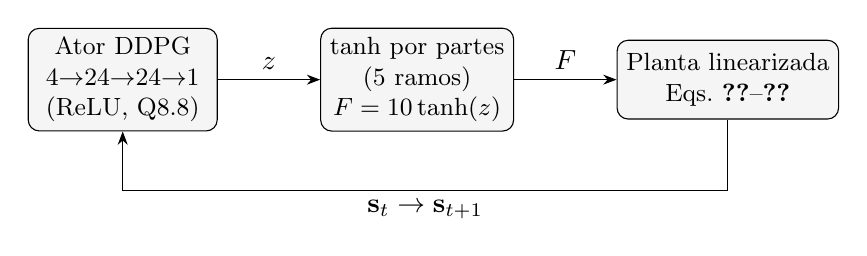
\begin{tikzpicture}[>=Stealth,
    blk/.style={draw,rounded corners,minimum height=1.0cm,minimum width=2.4cm,align=center,fill=black!4,font=\small}]
    \node[blk] (rede) {Ator DDPG\\$4{\to}24{\to}24{\to}1$\\(ReLU, Q8.8)};
    \node[blk,right=1.3cm of rede] (tanh) {$\tanh$ por partes\\(5 ramos)\\$F=10\tanh(z)$};
    \node[blk,right=1.3cm of tanh] (planta) {Planta linearizada\\Eqs.~\ref{eq:din1}--\ref{eq:din2}};
    \draw[->] (rede) -- node[above]{$z$} (tanh);
    \draw[->] (tanh) -- node[above]{$F$} (planta);
    \draw[->] (planta.south) -- ++(0,-0.9) -| node[pos=0.25,below]{$\mathbf{s}_t\to\mathbf{s}_{t+1}$} (rede.south);
  \end{tikzpicture}
  \legend{Fonte: elaborada pelo autor, 2026.}
\end{figure}

\section{Ponto fixo Q8.8 e divisão por termo}\label{sec:q88}

Cada valor real $v$ vira o inteiro $q(v)=\mathrm{round}(256\,v)$. O produto de dois valores Q8.8 tem escala $256^2$ e precisa ser dividido por 256. O ator implementa essa divisão \textbf{por termo}:
\[
  \mathrm{pre}_i = \Big\lfloor\tfrac{a\,x}{256}\Big\rfloor+\Big\lfloor\tfrac{b\,\dot x}{256}\Big\rfloor+\Big\lfloor\tfrac{c\,\theta}{256}\Big\rfloor+\Big\lfloor\tfrac{d\,\dot\theta}{256}\Big\rfloor+b_i,
\]
e não soma-depois-divide, porque os resultados diferem; e a divisão trunca a zero (como o \texttt{/} de C), não para $-\infty$ (como o \texttt{>>} aritmético), o que muda o resultado para valores negativos. A aproximação linear de $\tanh$ em cinco ramos satura em 255 (isto é, $\approx 1$) e limita $|F_Q|\le2550<2560$.

A rede tem $4{\cdot}24+24+24{\cdot}24+24+24+1=745$ parâmetros inteiros. O erro de quantização medido em 10\,000 estados (arquivo \texttt{quantization\_report.json}) é de até 7,76~N no pior caso, com média 0,078~N, percentil 95 de 0,23~N e percentil 99 de 1,09~N. A verificação é sobre o controlador \emph{quantizado}, que é o artefato executado.

\section{BMC e ESBMC}

No \emph{Bounded Model Checking} (BIERE et al., 1999), dado um programa, uma propriedade e um limite $K$, constrói-se uma fórmula $\Phi_K$ satisfatível se e somente se existe uma execução de até $K$ passos que viola a propriedade. O ESBMC (GADELHA et al., 2018) traduz programas C para fórmulas SMT. Satisfatível implica contraexemplo concreto; insatisfatível implica seguro \emph{até} $K$. A fórmula contém \textbf{$K$ cópias} da relação de transição, o que explica o crescimento de custo com $K$ (Seção~\ref{sec:parede}). As primitivas usadas nos \emph{harnesses} são \texttt{nondet\_int()} (variável simbólica), \texttt{\_\_ESBMC\_assume} (restringe o espaço) e \texttt{\_\_ESBMC\_assert} (propriedade).

\section{IC3/PDR}

O IC3 (BRADLEY, 2011), na implementação PDR do ABC (EÉN; MISHCHENKO; BRAYTON, 2011), mantém uma sequência de \emph{frames} $F_0,F_1,\dots$ que sobreaproximam os estados alcançáveis em até $i$ passos e os refina com cláusulas aprendidas, cada uma obtida por uma consulta SAT sobre \textbf{uma única cópia} da transição. Se dois \emph{frames} consecutivos coincidem, tem-se um \textbf{invariante indutivo}: o conjunto contém os estados iniciais, é fechado pela transição e não toca a região insegura. Isso prova segurança para todo $t$, sem horizonte. O IC3 pode não terminar: sem boa generalização das cláusulas, o número de \emph{frames} e de cláusulas cresce sem convergir.

\section{AIGER, bit-\emph{blasting} e nível de palavra}

O fluxo de síntese usa Yosys (WOLF; GLASER; KEPLER, 2013) e ABC (BRAYTON; MISHCHENKO, 2010): o Verilog é reduzido a um \emph{And-Inverter Graph} (AIG). Nessa forma cada palavra de 16 bits vira 16 bits independentes e a estrutura aritmética se perde; é uma hipótese deste trabalho, \textbf{não demonstrada}, que isso prejudique a generalização do IC3. Um motor em \emph{nível de palavra} (BTOR2: btormc, Pono, AVR, rIC3) preservaria a estrutura; nenhum deles foi executado aqui. Como substituto parcial usou-se o Z3/Spacer (resolvedor de cláusulas de Horn; KOMURAVELLI; GURFINKEL; CHAKI, 2014; DE MOURA; BJØRNER, 2008) sobre aritmética inteira exata.

\chapter{Parte I: o \emph{cart-pole} verificado com ESBMC}\label{cap:esbmc}

\section{Método}

\paragraph{Extração e geração de \emph{harnesses}.} Um \emph{pipeline} Python extrai os pesos do ator, quantiza em Q8.8, propaga intervalos de pré-ativação e emite um programa C sem laços: cada neurônio é uma linha, com ReLU como \texttt{pre > 0 ? pre : 0}. A ausência de laços permite \texttt{-{}-no-unwinding-assertions} sem perda de solidez.

\paragraph{Domínio de entrada.} Em Q8.8: $|x|\le614$ (2,4~m), $|\dot x|\le1280$ (5~m/s), $|\theta|\le53$ (12$^\circ$), $|\dot\theta|\le1280$ (5~rad/s), declarados por \texttt{\_\_ESBMC\_assume}.

\paragraph{Propriedades.} Quatro propriedades foram escritas para o ator DDPG:
\begin{itemize}
  \item \textbf{A} (direção): na zona de perigo ($\theta$ grande e $\dot\theta$ no mesmo sentido) o controlador empurra para o lado que corrige;
  \item \textbf{B} (segurança): a partir do domínio seguro, $|\theta|\le12^\circ$ após $N$ passos;
  \item \textbf{C} (limite de força): $|F_Q|\le2560$;
  \item \textbf{D} (não trivialidade): na zona de perigo o controlador aplica força de módulo mínimo (0,5~N).
\end{itemize}

\section{Resultados do ator DDPG}

A Tabela~\ref{tab:ddpg} reproduz o registro de execuções do ator DDPG com ESBMC 6.8.0.

\begin{table}[htb]
\caption{Verificação do ator DDPG com ESBMC 6.8.0: execução registrada.}\label{tab:ddpg}
\centering
\begin{tabular}{l|l|r|p{6.0cm}}
\toprule
\textbf{Propriedade} & \textbf{Veredito} & \textbf{Tempo} & \textbf{Contraexemplo / observação} \\
\midrule
A (lado direito)    & Contraexemplo & 1888 s & $x{=}-0{,}0117$, $\dot x{=}-4{,}92$, $\theta{=}0{,}109$, $\dot\theta{=}0$ \\
A (lado esquerdo)   & Contraexemplo & 2722 s & $z=27$ (força positiva com $\theta<-5{,}7^\circ$) \\
B (1 passo)         & Contraexemplo & 90 s   & $x{=}-0{,}754$, $\dot x{=}-3{,}92$, $\theta{=}-0{,}184$, $\dot\theta{=}-1{,}52$ (propriedade vacua; \S\ref{sec:vac}) \\
C (limite de força) & Provado       & 24 s   & vale por construção do $\tanh$ (\S\ref{sec:vac}) \\
\bottomrule
\end{tabular}
\legend{Fonte: \texttt{cartpole/ddpg\_closed\_loop\_results.json}. Execução anterior às correções da \S\ref{sec:vac}; a propriedade D não tem resultado armazenado nesse arquivo.}
\end{table}

\paragraph{Leitura do contraexemplo de A.} O ESBMC encontrou estados em que a rede aplica a força contrária à esperada, o que é uma violação da propriedade \emph{como especificada}. Uma ressalva: $z>0$ não implica $F>0$, pois a divisão inteira do primeiro ramo do $\tanh$ dá $\lfloor 1\cdot252/256\rfloor=0$; logo $z=1$ resulta em força nula. A propriedade A é, portanto, ao mesmo tempo restritiva e frouxa; a propriedade D foi criada para cobrir a lacuna.

\section{Propriedades vacuas e sua correção}\label{sec:vac}

Duas propriedades originais não dependiam do controlador, o que foi descoberto ao executar o mesmo \emph{assert} sem a rede:

\begin{enumerate}
  \item \textbf{B de um passo.} O valor asseriado era $\theta_{novo}=\theta+5\dot\theta/256$, que \emph{não contém} $F$ (Equações~\ref{eq:din1}--\ref{eq:din2}: a força só chega a $\theta$ via $\dot\theta$, no passo seguinte). Executando sem rede e com $F_Q$ arbitrário, o veredito e o contraexemplo ($\theta=53$, $\dot\theta=64\to\theta_{novo}=54$) se reproduzem idênticos: os 745 pesos eram código morto. \textbf{Correção:} B passou a dois passos, asserindo $\theta_2=\theta_{novo}+5\dot\theta_{novo}/256$. Dependência confirmada: com $F_Q$ livre o contraexemplo é $\theta_2=79$; com $F_Q=0$ é $\theta_2=55$.
  \item \textbf{C.} $|F_Q|\le2560$ vale por construção, pois o $\tanh$ por partes satura em 255 e $255\cdot10=2550$. Substituindo a rede inteira por $z$ livre, a prova passa em 0,72~s. \textbf{Correção:} C foi reclassificada como \emph{sanidade da quantização}, e D foi criada para depender dos pesos.
\end{enumerate}

Este é um resultado metodológico: duas das três provas originais eram vazias, e só foi possível saber isso ao isolar a propriedade da rede.

\section{Envelope de segurança em dois passos}\label{sec:envelope}

\begin{table}[htb]
\caption{Segurança em dois passos em função do limite de $|\dot\theta|$ inicial.}\label{tab:env}
\centering
\begin{tabular}{r|r|l|r}
\toprule
$|\dot\theta|\le$ (Q8.8) & rad/s & Veredito & Tempo \\
\midrule
1280 & 5,00 & Contraexemplo & 25,4 s \\
 640 & 2,50 & Contraexemplo & 28,8 s \\
 320 & 1,25 & Indeciso & $>$300 s \\
 160 & 0,62 & Indeciso & $>$300 s \\
  80 & 0,31 & Indeciso & $>$300 s \\
\bottomrule
\end{tabular}
\legend{Fonte: capítulo de resultados do artigo do projeto (\texttt{artigo/caps/4resultados.tex}, Tabela~\texttt{envelope}).}
\end{table}

Conclusão defensável: a segurança de dois passos é \textbf{violada} para $|\dot\theta|\ge2{,}5$~rad/s e \textbf{indecisa} abaixo disso. Não se conclui que o controlador seja seguro nas caixas estreitas. O comportamento é contraintuitivo: \emph{reduzir a região inicial torna o problema mais difícil}. Com caixa larga existe contraexemplo, e achá-lo é a direção barata (SAT); com caixa estreita é preciso \emph{provar} que não existe, e a prova (UNSAT) é cara.

\section{A parede do BMC}\label{sec:parede}

A Tabela~\ref{tab:parede} e a Figura~\ref{fig:parede} mostram a medição com uma rede de 24 neurônios.

\begin{table}[htb]
\caption{Custo do BMC em função do horizonte $K$.}\label{tab:parede}
\centering
\begin{tabular}{r|r|r}
\toprule
$K$ & Tempo & Memória \\
\midrule
1 & 0,3 s & 46 MB \\
2 & 77 s  & 137 MB \\
4 & 909 s & 383 MB \\
\bottomrule
\end{tabular}
\legend{Fonte: cabeçalho de \texttt{ic3/gen\_transition\_system.py}.}
\end{table}

\begin{figure}[htb]
  \caption{Tempo do BMC (ESBMC) versus horizonte $K$, escala logarítmica.}\label{fig:parede}
  \centering
  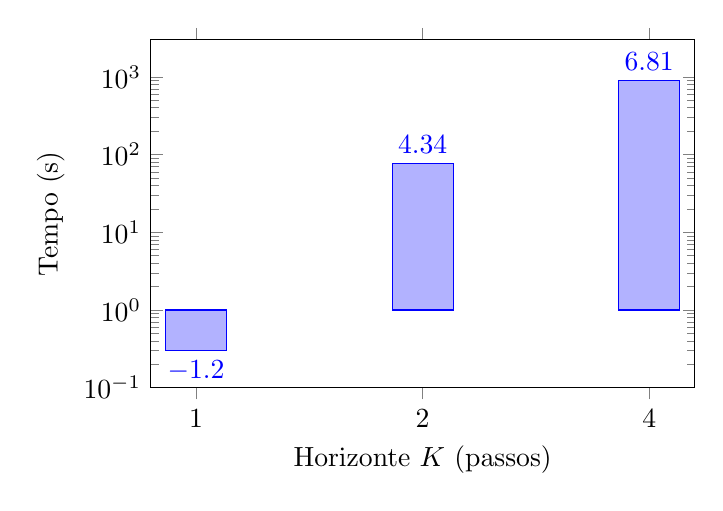
\begin{tikzpicture}
    \begin{axis}[ybar,ymode=log,width=0.7\textwidth,height=6cm,
      xlabel={Horizonte $K$ (passos)},ylabel={Tempo (s)},
      symbolic x coords={1,2,4},xtick=data,ymin=0.1,ymax=3000,
      nodes near coords,bar width=22pt]
      \addplot coordinates {(1,0.3) (2,77) (4,909)};
    \end{axis}
  \end{tikzpicture}
  \legend{Fonte: Tabela~\ref{tab:parede}.}
\end{figure}

O \emph{harness} de 50 passos nunca foi concluído por esse motivo: a parede está em $K{=}4$, não em 50. A causa é estrutural (uma única fórmula com $K$ cópias da transição), não de esforço.

\section{Propriedades estruturais da rede}

Perguntou-se ao ESBMC se algum neurônio é \emph{morto} (ReLU nunca ativa) ou \emph{saturado}. No ator DDPG, o registro (\texttt{ddpg\_dead\_neuron\_results.json}, \texttt{ddpg\_saturation\_results.json}) indica: \textbf{nenhum dos 48 neurônios é morto} (24 por camada, sem \emph{timeouts}), nenhum neurônio da camada~1 é saturado e a saída é responsiva. Ressalva: na camada~2 a entrada $h_1$ é tratada como caixa relaxada (não o valor calculado a partir do estado); assim, ``vivo'' na camada~2 deve ser lido com cautela e o resultado firme vale para a camada~1.

\section{O controlador DQN, para comparação}

O projeto também verificou um controlador DQN (\texttt{closed\_loop\_results.json}). A propriedade A obteve contraexemplo no lado esquerdo ($x{=}-1{,}246$, $\dot x{=}3{,}52$, $\theta{=}-0{,}191$, $\dot\theta{=}-0{,}42$, ação~1) e \emph{timeout} no lado direito. A segurança de um passo (B) obteve contraexemplo em $\dot\theta=-4{,}59$~rad/s, um valor extremo em que $\theta$ cruza o limite em um passo independentemente da ação, o que \emph{reforça} o achado de vacuidade da Seção~\ref{sec:vac}.

\section{Síntese da Parte I}

O ESBMC \textbf{decide} propriedades locais (neurônios, limites, um e dois passos com caixas largas) e produz contraexemplos concretos, reproduzíveis no simulador. Ele \textbf{não decide} (i) a segurança de dois passos em caixas estreitas e (ii) horizontes $K\gtrsim4$. A prova de segurança para $t\to\infty$ está fora do alcance do método nesta formulação, o que motiva a rota indutiva do capítulo seguinte.

\chapter{Parte II: a rota IC3/PDR}\label{cap:ic3}

\section{Do C ao sistema de transição}

O IC3 exige um sistema de transição. A malha fechada foi exportada para Verilog (\texttt{gen\_transition\_system.py}), com quatro registradores de estado de 16 bits (mais um \emph{flag} \texttt{started}, 65 \emph{latches} no total), as mesmas expressões do ator e da dinâmica, e:
\begin{itemize}
  \item \textbf{estado inicial}: caixa $|\text{estado}|\le5$ em Q8.8 ($\approx0{,}02$), obtida por \emph{clamp} das entradas livres no primeiro ciclo;
  \item \textbf{propriedade}: $\lnot\,\texttt{bad}$, com $\texttt{bad}=(\theta>53)\lor(\theta<-53)$;
  \item o próximo estado é \textbf{truncado} em 16 bits (\texttt{n\_x[15:0]}).
\end{itemize}
Uma diferença deliberada em relação ao \emph{harness} C: os \texttt{\_\_ESBMC\_assume} de limite por neurônio são \textbf{omitidos}, pois são uma muleta do BMC (podam o espaço); nenhum estado alcançável é descartado.

\begin{figure}[htb]
  \caption{As duas rotas de verificação a partir do mesmo ator quantizado.}\label{fig:rotas}
  \centering
  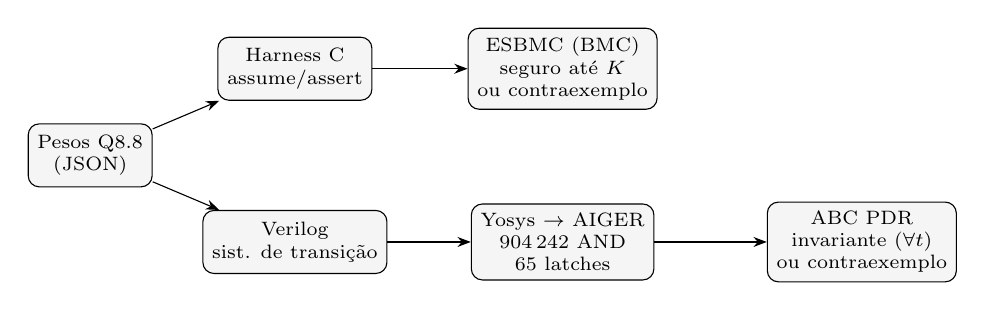
\begin{tikzpicture}[>=Stealth,
    blk/.style={draw,rounded corners,minimum height=0.8cm,align=center,fill=black!4,font=\scriptsize}]
    \node[blk] (w) at (0,0) {Pesos Q8.8\\(JSON)};
    \node[blk] (c) at (2.6,1.1) {Harness C\\assume/assert};
    \node[blk] (esbmc) at (6.0,1.1) {ESBMC (BMC)\\seguro até $K$\\ou contraexemplo};
    \node[blk] (v) at (2.6,-1.1) {Verilog\\sist. de transição};
    \node[blk] (aig) at (6.0,-1.1) {Yosys $\to$ AIGER\\904\,242 AND\\65 latches};
    \node[blk] (pdr) at (9.8,-1.1) {ABC PDR\\invariante ($\forall t$)\\ou contraexemplo};
    \draw[->] (w) -- (c); \draw[->] (c) -- (esbmc);
    \draw[->] (w) -- (v); \draw[->] (v) -- (aig); \draw[->] (aig) -- (pdr);
  \end{tikzpicture}
  \legend{Fonte: elaborada pelo autor, 2026.}
\end{figure}

\section{Resultados sobre o ator real}

\begin{table}[htb]
\caption{BMC e IC3 sobre a malha fechada.}\label{tab:bmcic3}
\centering
\begin{tabular}{p{2.0cm}|p{3.2cm}|p{3.3cm}|r|r}
\toprule
\textbf{Método} & \textbf{Modelo} & \textbf{Veredito} & \textbf{Tempo} & \textbf{Memória} \\
\midrule
BMC (ESBMC)  & sintético, $K{=}4$         & Seguro até 4 passos           & 909 s  & 383 MB \\
IC3 (ABC)    & sintético com batente (histórico) & \textbf{Provado} $\forall t$ & 0,37 s & trivial \\
IC3 (ABC)    & ator DDPG real             & Indeciso (\emph{frame}~2)     & 1802 s & 577 MB \\
BMC (ABC)    & ator DDPG real             & Indeciso (5 \emph{frames})    & 901 s  & 503 MB \\
Spacer (Z3)  & ator DDPG real, inteiros   & Indeciso                      & 1800 s & --- \\
\bottomrule
\end{tabular}
\legend{Fonte: \texttt{ic3/EVIDENCIA.md}; \texttt{ic3/validacao/real/}. O modelo sintético com batente e seu log não estão no repositório atual e \textbf{não foram reexecutados}; é resultado histórico. A reexecução do PDR real mediu pico de 577~MB (o registro anterior citava 708~MB).}
\end{table}

\paragraph{O sucesso sintético.} No modelo sintético com batente mecânico, o IC3 provou segurança ilimitada em 0,37~s com um invariante de quatro cláusulas sobre três dos 65 bits de estado: ele ignorou a rede e usou só a estrutura do batente. Nenhum BMC produz esse tipo de resultado. Mas, justamente porque a segurança vem da física imposta e não do controlador, esse resultado demonstra a capacidade do método, não a segurança do ator.

\paragraph{O ator real.} Nenhum motor decide. O log bruto do PDR (Apêndice~\ref{ap:log}) mostra que o ABC parou no \emph{frame}~2 com 22 cláusulas e 106 chamadas SAT. Só 42,2~s (2,34\%) dos 1801~s foram contabilizados em chamadas SAT concluídas. A interpretação, uma \textbf{hipótese não medida por chamada}, é que o gargalo é uma única consulta SAT sobre a transição, que nunca termina, e não a convergência do IC3.

\section{Comparação controlada sobre a mesma instância}

Para separar o efeito do tamanho do efeito do método, geraram-se redes aleatórias (pesos de semente fixa~7) de arquitetura $4{\to}H{\to}H{\to}1$ e rodaram-se os três motores por 300~s cada (Tabela~\ref{tab:escala}, Figura~\ref{fig:escala}).

\begin{table}[htb]
\caption{Comparação controlada, mesma instância, 300 s por motor.}\label{tab:escala}
\centering
\begin{tabular}{r|r|c|c|c}
\toprule
$H$ & Portas AND & PDR (ABC) & BMC (ABC \texttt{bmc3}) & Spacer (Z3) \\
\midrule
 4 &  61\,359 & indeciso & 9 \emph{frames} & indeciso \\
 8 & 143\,721 & indeciso & 5 \emph{frames} & indeciso \\
12 & 272\,044 & indeciso & 5 \emph{frames} & indeciso \\
16 & 430\,346 & indeciso & 5 \emph{frames} & indeciso \\
24 (real) & 904\,242 & indeciso (1800 s) & 5 \emph{frames} (901 s) & indeciso (1800 s) \\
\bottomrule
\end{tabular}
\legend{Fonte: \texttt{ic3/validacao/RESULTADOS.md}. Pesos aleatórios: não se sabe se essas instâncias são seguras.}
\end{table}

\begin{figure}[htb]
  \caption{Tamanho do problema (portas AND do AIG) versus largura $H$ das camadas ocultas.}\label{fig:escala}
  \centering
  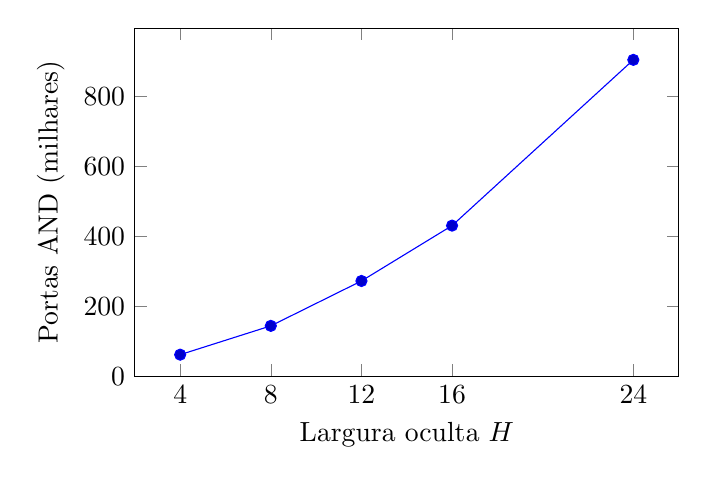
\begin{tikzpicture}
    \begin{axis}[width=0.7\textwidth,height=6cm,xlabel={Largura oculta $H$},ylabel={Portas AND (milhares)},
      xtick={4,8,12,16,24},ymin=0]
      \addplot+[mark=*] coordinates {(4,61.359) (8,143.721) (12,272.044) (16,430.346) (24,904.242)};
    \end{axis}
  \end{tikzpicture}
  \legend{Fonte: Tabela~\ref{tab:escala}. O tamanho cresce aproximadamente com $H^2$.}
\end{figure}

\paragraph{O que a Tabela~\ref{tab:escala} diz.} Nenhum dos três motores decide nem a menor rede ($H{=}4$, 61\,mil portas). Portanto a dificuldade \emph{não} é só de tamanho: variar $H$ de 4 a 24 não muda o veredito. Este é um resultado negativo sobre os motores e a codificação, e uma advertência: o sucesso sintético \textbf{não} se generaliza por escala.

\chapter{Validação do pipeline}\label{cap:valid}

Uma prova de segurança é tão confiável quanto a tradução que a produziu. Este capítulo mede o quanto o pipeline Verilog$\to$AIGER é confiável.

\section{Fidelidade da tradução}

\subsection{O lema da divisão}

O gerador implementa a divisão por 256 como \texttt{td(v) = v[31] ? -((-v)>{}>{}>8) : (v>{}>{}>8)}. Um problema SAT sobre todos os $v$ de 32 bits compara \texttt{td} com o \texttt{v/256} do C. O resultado é \textbf{uma única divergência}: $v=-2^{31}$, onde \texttt{td} dá $+8\,388\,608$ e o C dá $-8\,388\,608$ (a negação de $-2^{31}$ transborda). Para todos os outros valores as duas coincidem.

\subsection{Análise de intervalos}

Calculou-se, com aritmética de intervalos em inteiros, o intervalo de \textbf{759 expressões} do ator para estado de 16 bits e entrada arbitrária. O maior valor absoluto é $1{,}81\times10^9<2^{31}\approx2{,}15\times10^9$: \textbf{nenhum estouro de 32 bits e nenhum argumento de \texttt{td} pode ser $-2^{31}$}. Logo a única divergência do lema é inalcançável. Com estado de 32 bits (variante \texttt{-{}-bits 32}), em contraste, 749 das 759 expressões podem estourar, de modo que essa variante \textbf{não} é fiel ao \texttt{int} do C.

\subsection{Equivalência por SAT}

O \emph{miter} monolítico (gerador $\equiv$ referência com \texttt{/}) tem 9\,736\,668 variáveis e 28\,860\,715 cláusulas e \textbf{não terminou em 3000~s}. Um \emph{miter} \emph{composicional} (um por neurônio, com entradas livres restritas aos intervalos calculados) provou \textbf{49 de 50 blocos equivalentes}: os 24 neurônios da camada~1, os 24 da camada~2 e a saída. O bloco \texttt{TANH\_DIN} (o $\tanh$ de cinco ramos mais a dinâmica, que mistura cinco divisões) estourou 600~s: \textbf{indeciso}. Assim, a equivalência formal da rede está provada; a do $\tanh$/dinâmica está apenas \emph{amostrada} e sustentada por intervalos.

\begin{table}[htb]
\caption{Resumo da fidelidade da tradução.}\label{tab:fid}
\centering
\begin{tabular}{p{7.2cm}|p{5.6cm}}
\toprule
\textbf{Verificação} & \textbf{Resultado} \\
\midrule
\texttt{td} vs \texttt{/256}, todo $v$ de 32 bits & divergente só em $v=-2^{31}$ \\
Intervalos, 759 expressões, estado de 16 bits & máx.\ $1{,}81\times10^9$; sem estouro; $-2^{31}$ inalcançável \\
Intervalos, estado de 32 bits & 749 podem estourar: variante infiel \\
\emph{Miter} SAT monolítico & indeciso (3000 s) \\
\emph{Miter} SAT composicional & 49/50 provados; \texttt{TANH\_DIN} indeciso \\
Teste diferencial por amostragem & coincide (não é prova universal) \\
\bottomrule
\end{tabular}
\legend{Fonte: \texttt{ic3/validacao/RESULTADOS.md}.}
\end{table}

\paragraph{Lacuna que permanece.} O estado é truncado em 16 bits. A \textbf{ausência de \emph{wrap} nos estados alcançáveis} não foi provada; sem ela, uma prova de segurança seria sobre o modelo truncado, não sobre o \texttt{int} do C.

\section{Teste de mutação: o pipeline sabe reprovar?}

Se um verificador só devolve ``indeciso'', nada se sabe sobre sua capacidade de reprovar. Criaram-se mutantes do ator real com insegurança \emph{conhecida} e rodou-se o PDR (limite de 300~s):

\begin{table}[htb]
\caption{Mutantes do ator real.}\label{tab:mut}
\centering
\begin{tabular}{p{3.6cm}|p{4.2cm}|p{3.0cm}|r}
\toprule
\textbf{Mutante} & \textbf{Insegurança conhecida} & \textbf{Veredito} & \textbf{Tempo} \\
\midrule
m5: $\theta$ inicial livre & sim, profundidade 0 & Contraexemplo & 3,5 s \\
m1: $\dot\theta$ inicial livre & sim, profundidade 1 ($\theta_1=\theta_0+640>53$) & Contraexemplo & 6,9 s \\
m3: controle desligado & sim, instável em malha aberta & Contraexemplo & 42,2 s \\
m2: atuador invertido & não sabida & Indeciso & 302 s \\
m4: limite $|\theta|\le6$ & \textbf{inválido}: o controlador pode manter $|\theta|\le6$ & Indeciso & 308 s \\
\bottomrule
\end{tabular}
\legend{Fonte: \texttt{ic3/validacao/mut/}. m2 e m4 não têm verdade conhecida e não contam como teste.}
\end{table}

O ABC \textbf{reprova os três mutantes comprovadamente inseguros}. O pipeline, portanto, não só ``não prova'': ele acha contraexemplos quando existem em profundidade pequena ou média (para m3, no \emph{frame}~77). Sobre m4: foi criado esperando-se insegurança, mas o controlador pode de fato mantê-lo; foi reclassificado como inválido em vez de contado.

\section{Motor independente em nível de palavra}

O Z3/Spacer, com aritmética inteira exata (sem bit-\emph{blasting}), foi aplicado ao ator real (1800~s) e aos mutantes (400~s). Resultado: \textbf{indeciso em todos}, inclusive em m1, cujo contraexemplo tem profundidade~1. É um resultado negativo sobre \emph{esta} codificação e versão (Z3 4.8.12); não se estende a Pono, AVR, btormc ou rIC3, que não foram testados. A hipótese de que ``o gargalo é o bit-\emph{blasting}'' \textbf{não ganhou suporte}: mudar para nível de palavra com o Z3 não ajudou, e a dificuldade parece estar na consulta de um passo (ReLU mais divisão truncada).

\chapter{Discussão: o que está provado e quão novo é}\label{cap:disc}

\section{Balanço de evidência}

\begin{table}[htb]
\caption{O que está estabelecido, o que está refutado e o que está aberto.}\label{tab:balanco}
\centering
\begin{tabular}{p{6.0cm}|p{2.7cm}|p{4.2cm}}
\toprule
\textbf{Afirmação} & \textbf{Estado} & \textbf{Evidência} \\
\midrule
Ator real é seguro $\forall t$ (IC3) & \textbf{Aberto} & PDR indeciso (frame 2, 1800 s) \\
Ator real é seguro em 2 passos, caixa larga & \textbf{Refutado} & contraexemplo em 25--29 s (ESBMC) \\
Pipeline reprova modelo inseguro & \textbf{Estabelecido} (3 mutantes) & Tabela~\ref{tab:mut} \\
Rede equivalente ao C (por bloco) & \textbf{49/50 provado} & \emph{miter} composicional \\
Tradução sem \emph{wrap} de 16 bits & \textbf{Aberto} & não provado \\
Planta e região inicial = planta real & \textbf{Aberto} & não validado \\
Prova não trivial (sem batente) & \textbf{Aberto} & não obtida \\
IC3 supera BMC no ator real & \textbf{Não estabelecido} & ambos indecisos \\
\bottomrule
\end{tabular}
\legend{Fonte: elaborada pelo autor, 2026.}
\end{table}

\section{Isto é revolucionário?}

\textbf{Ainda não, e este relatório não o afirma.} O resultado positivo (prova ilimitada em 0,37~s) vale para um modelo sintético com batente. No ator real a técnica não decide, nem o BMC, nem o Spacer. A literatura já tem verificação de redes quantizadas por SMT/BMC, por programação linear inteira, \emph{model checking} neural e verificação de C via BTOR2/IC3; encontrei referências a esses temas apenas por títulos e trechos (por exemplo arXiv 2106.05997 sobre redes quantizadas, e Giacobbe et al., NeurIPS 2024), \textbf{sem leitura}. Numa busca curta não achei IC3 sobre malha fechada planta mais rede, mas ausência na busca não é ausência na literatura. Falta uma revisão sistemática e a comparação com verificadores dedicados (Marabou, NNV, $\alpha,\beta$-CROWN), que usam propagação de limites e \emph{branch-and-bound}.

O que \emph{já} é contribuição defensável: (i) o método de isolar a propriedade da rede para detectar vacuidade (duas de três provas originais eram vazias); (ii) a cadeia de validação, com mutantes de verdade conhecida e \emph{miters} composicionais; (iii) o registro honesto dos resultados negativos.

\section{Ameaças à validade}

\begin{itemize}
  \item \textbf{Planta.} A dinâmica é linearizada e o estado inicial é uma caixa pequena; ambos não foram validados contra a planta real.
  \item \textbf{Tradução.} Estado de 16 bits truncado; ausência de \emph{wrap} alcançável não provada; \texttt{TANH\_DIN} não provado equivalente.
  \item \textbf{Comparação.} ESBMC (registros do repositório) e ABC/Spacer (reexecuções) não compartilham máquina; tempos absolutos não se comparam.
  \item \textbf{Escala.} A comparação controlada usa pesos aleatórios de segurança desconhecida.
  \item \textbf{Histórico.} O modelo sintético com batente e seu log não estão no repositório atual.
\end{itemize}

\chapter{Conclusão}\label{cap:concl}

O ESBMC (BMC) decide propriedades locais e de curto horizonte do controlador DDPG quantizado e produz contraexemplos concretos e reproduzíveis, mas esbarra numa parede estrutural em $K\approx4$ e não decide segurança para horizonte ilimitado. A rota IC3/PDR gera uma prova ilimitada num modelo com batente mecânico, mas não decide o ator real; um motor em nível de palavra (Z3/Spacer) também não. O pipeline foi validado quanto à tradução (intervalos e SAT composicional, 49/50 blocos) e quanto à capacidade de reprovar (três mutantes inseguros detectados), e as lacunas restantes estão enumeradas.

\paragraph{Próximos passos, em ordem de custo--benefício.}
\begin{enumerate}
  \item dividir \texttt{TANH\_DIN} por ramo para fechar a equivalência formal;
  \item provar a ausência de \emph{wrap} de 16 bits nos estados alcançáveis, ou inserir um guarda de estouro na propriedade \texttt{bad};
  \item executar um motor BTOR2 em nível de palavra (btormc, Pono, AVR, rIC3) sobre o mesmo modelo;
  \item obter uma prova não trivial: invariante sem batente em modelo reduzido;
  \item comparar com Marabou/NNV/$\alpha,\beta$-CROWN e fazer a revisão sistemática de literatura;
  \item validar a planta linearizada e a região inicial contra a planta não linear.
\end{enumerate}

\begin{apendicesenv}
\partapendices

\chapter{Logs brutos selecionados}\label{ap:log}

\section{PDR no ator real (excerto de \texttt{real/cl\_ddpg16.abc.out})}
\begin{lstlisting}
ABC command line: "read_aiger cl_ddpg16.aig; pdr -v -T 1800".
Frame Clauses                                  Max Queue Flops Cex      Time
  1 : 0 21                                                1    14      1.50 sec
  2 : 0 14 8                                              2    16   1800.89 sec
Reached timeout (1800 seconds) in frame 2.
Block =   22  Oblig =    25  Clause =    22  Call =   106 (sat=61.3%)  Cex =   0
SAT solving =    42.18 sec (  2.34 %)
Property UNDECIDED.  Time =  1801.36 sec
\end{lstlisting}

\section{Resumo do \emph{wrapper} (\texttt{real/run\_pdr.stdout.txt})}
\begin{lstlisting}
i/o = 65/1  lat = 65  and = 904242  lev = 689
Reached timeout (1800 seconds) in frame 2.
status=INCONCLUSIVO  tempo=1802.6s  pico_RSS=577MB
\end{lstlisting}

\section{Contraexemplo do lema da divisão (\texttt{lema\_td.cex.txt})}
\begin{lstlisting}
SAT proof finished - model found: FAIL!
  \a                  8388608    800000   00000000100000000000000000000000
  \b                 -8388608  ff800000   11111111100000000000000000000000
  \v              -2147483648  80000000   10000000000000000000000000000000
\end{lstlisting}

\section{Mutante detectado (\texttt{mut/mutantes.saida.txt})}
\begin{lstlisting}
### m3_controle_desligado
Output 0 of miter "m3_controle_desligado" was asserted in frame 77.  Time = 42.18 sec
status=CONTRAEXEMPLO  tempo=42.2s  pico_RSS=63MB
\end{lstlisting}

\chapter{Reprodução}

Os \emph{scripts} e logs estão em \texttt{pibic/ic3/} e \texttt{pibic/ic3/validacao/}. A imagem de ferramentas é construída pelo \texttt{Dockerfile} da pasta de validação (Ubuntu 24.04, Yosys, Z3). Exemplos:

\begin{lstlisting}
python3 gen_transition_system.py --bits 16 -o cl_ddpg16.v
python3 validate_forward.py -n 12
./run_pdr.sh cl_ddpg16.v 1800     # 0 prova, 1 cex, 2 erro, 3 indeciso
\end{lstlisting}
\end{apendicesenv}

\begin{thebibliography}{99}
\bibitem{barto} BARTO, A. G.; SUTTON, R. S.; ANDERSON, C. W. Neuronlike adaptive elements that can solve difficult learning control problems. \emph{IEEE Trans. Systems, Man, and Cybernetics}, v. 13, n. 5, p. 834--846, 1983.
\bibitem{biere} BIERE, A. et al. Symbolic model checking without BDDs. In: \emph{TACAS}, 1999.
\bibitem{gadelha} GADELHA, M. R. et al. ESBMC 5.0: an industrial-strength C model checker. In: \emph{ASE}, 2018.
\bibitem{bradley} BRADLEY, A. R. SAT-based model checking without unrolling. In: \emph{VMCAI}, 2011.
\bibitem{een} EÉN, N.; MISHCHENKO, A.; BRAYTON, R. Efficient implementation of property directed reachability. In: \emph{FMCAD}, 2011.
\bibitem{brayton} BRAYTON, R.; MISHCHENKO, A. ABC: a system for sequential synthesis and verification. In: \emph{CAV}, 2010.
\bibitem{wolf} WOLF, C.; GLASER, J.; KEPLER, J. Yosys: a free Verilog synthesis suite. In: \emph{Austrochip}, 2013.
\bibitem{komuravelli} KOMURAVELLI, A.; GURFINKEL, A.; CHAKI, S. SMT-based model checking for recursive programs. In: \emph{CAV}, 2014.
\bibitem{demoura} DE MOURA, L.; BJØRNER, N. Z3: an efficient SMT solver. In: \emph{TACAS}, 2008.
\end{thebibliography}

\end{document}
